\documentclass[11pt]{article}

\usepackage[margin=0.72in]{geometry}
\usepackage{graphicx}
\usepackage{booktabs}
\usepackage{tabularx}
\usepackage{array}
\usepackage{amsmath}
\usepackage{caption}
\usepackage{subcaption}
\usepackage{float}
\usepackage{xcolor}
\usepackage{hyperref}
\usepackage{listings}
\usepackage{appendix}

\hypersetup{
  colorlinks=true,
  linkcolor=blue!45!black,
  citecolor=blue!45!black,
  urlcolor=blue!45!black
}

\captionsetup{font=small, labelfont=bf}
\setlength{\parskip}{0.35em}
\setlength{\parindent}{0pt}
\renewcommand{\arraystretch}{1.08}

\lstset{
  basicstyle=\ttfamily\scriptsize,
  breaklines=true,
  frame=single,
  columns=fullflexible,
  keepspaces=true,
  showstringspaces=false,
  keywordstyle=\color{blue!60!black},
  commentstyle=\color{green!35!black},
  literate={─}{-}1 {→}{$\to$}1 {←}{$\leftarrow$}1 {⇒}{$\Rightarrow$}1
           {Σ}{$\Sigma$}1 {·}{.}1 {₀}{$_0$}1 {₁}{$_1$}1
           {α}{$\alpha$}1 {≈}{$\approx$}1 {∈}{$\in$}1
}

\title{\vspace{-1.4cm}\textbf{Do Languages Minimise Complex Interveners?}\\
\large A Cross-Linguistic Test Using Universal Dependencies}
\author{Aditya, Anya, Devansh, Nitika, Pubali, Sidhant, Srishti, and Suneet}
\date{CGS410: Language in the Mind and Machine}

\begin{document}
\maketitle
\vspace{-0.6cm}

\begin{abstract}
Dependency Length Minimization (DLM) says that languages prefer to keep syntactically related words close together. A stronger processing-based idea is \emph{Intervener Complexity Minimization} (ICM): when a dependency is long, the words between the head and dependent should themselves be syntactically simple. We test this idea in 12 Universal Dependencies treebanks by extracting every token that intervenes between a dependency head and dependent. Complexity is measured by whether the intervener is a syntactic head, its number of direct children, its subtree size, and its attachment relation. We compare the observed distributions with a random-word-order baseline that keeps each dependency tree fixed. Across 9,012,884 real intervener observations and 22,329,108 baseline observations, all 12 languages have significantly lower intervener head-rate, arity, and subtree size than expected under random linearisation. The results support ICM as a cross-linguistic pressure on word order.
\end{abstract}

\section{Motivation for the Research Problem}
Human sentence processing is limited by memory. When two syntactically related words are far apart, the listener or reader must keep one word active while processing the intervening material. DLM predicts that languages reduce this burden by shortening dependencies \cite{gibson1998linguistic,liu2008dependency}. However, distance alone may not capture the whole processing cost. A five-word gap filled with simple function words may be easier than a five-word gap filled with syntactically complex phrases.

This project asks whether natural languages reduce not only the \emph{length} of dependencies, but also the \emph{complexity} of the material inside long dependencies. We follow the basic idea of Yadav, Mittal, and Husain \cite{yadav2022reappraisal}: for a dependency arc from head $h$ to dependent $d$, every token $k$ whose linear position lies strictly between them is an intervener:
\[
I(h,d)=\{k:\min(pos(h),pos(d))<pos(k)<\max(pos(h),pos(d))\}.
\]
Our main research question is: \textbf{Are intervening tokens in real languages syntactically simpler than they would be under random word order?} The objective is to test this question across a typologically diverse sample of 12 languages, using a single extraction and inference pipeline.

\section{Hypotheses and Predictions}
\textbf{H1: Intervener Complexity Minimization.} Real word orders should place fewer syntactic heads inside dependency spans than a random baseline that preserves the same dependency trees. The primary prediction is:
\[
\Pr(\text{arity}(k)>0 \mid k\in I)_{\text{real}}
<
\Pr(\text{arity}(k)>0 \mid k\in I)_{\text{baseline}}.
\]

\textbf{H2: Simpler intervening structure.} Real interveners should also have lower arity and smaller subtree size than baseline interveners. This predicts one-tailed Mann--Whitney U tests in the direction real $<$ baseline.

\textbf{H3: Distributional difference.} The full distributions of intervener part of speech, arity, and subtree size should differ from the random baseline. This predicts non-zero Jensen--Shannon divergence (JSD), especially for arity and subtree size.

\section{Methods}
\textbf{Data.} We used 12 Universal Dependencies treebanks: English, German, Spanish, Russian, Arabic, Hindi, Turkish, Finnish, Japanese, Chinese, Basque, and Ancient Greek. The sample covers different language families and word-order profiles. All train/dev/test CoNLL-U files available in each treebank were used. The final statistical comparison contains 9.01M real intervener observations and 22.33M baseline observations.

\textbf{Feature extraction.} For every non-adjacent dependency arc, we extracted all intervening tokens. For each intervener we recorded: (A) UPOS tag, (B) arity, defined as the number of direct UD children, (C) subtree size, defined as the number of tokens dominated by the intervener, and (D) whether the intervener attaches to the arc head, the dependent, or neither. The main ICM metric is \emph{head-rate}: the proportion of interveners with arity $>0$.

\textbf{Random baseline.} The null model randomly permutes word order inside each sentence while keeping the dependency tree fixed. We then re-extract interveners with the same procedure. This baseline asks what the intervener distribution would look like if the tree structure were unchanged but linear order did not minimise complexity.

\textbf{Inference.} We used three tests. First, head-rate was compared with a one-tailed two-proportion z-test. Second, arity and subtree-size samples were compared with one-tailed Mann--Whitney U tests, testing whether real values are stochastically smaller than baseline values. Third, JSD was used to quantify distributional distance:
\[
JSD(P,Q)=\frac{1}{2}KL(P\Vert M)+\frac{1}{2}KL(Q\Vert M),\quad M=\frac{1}{2}(P+Q).
\]
The significance threshold was Bonferroni-corrected over 12 languages: $\alpha=0.05/12=0.0042$.

\section{Results}
The main prediction is supported in every language. Mean real head-rate is 0.294, while mean baseline head-rate is 0.367. The average real-baseline difference is $-0.073$, with all languages showing lower real head-rate than baseline. The smallest reduction is German ($-0.046$) and the largest is Japanese ($-0.116$).

\begin{figure}[H]
  \centering
  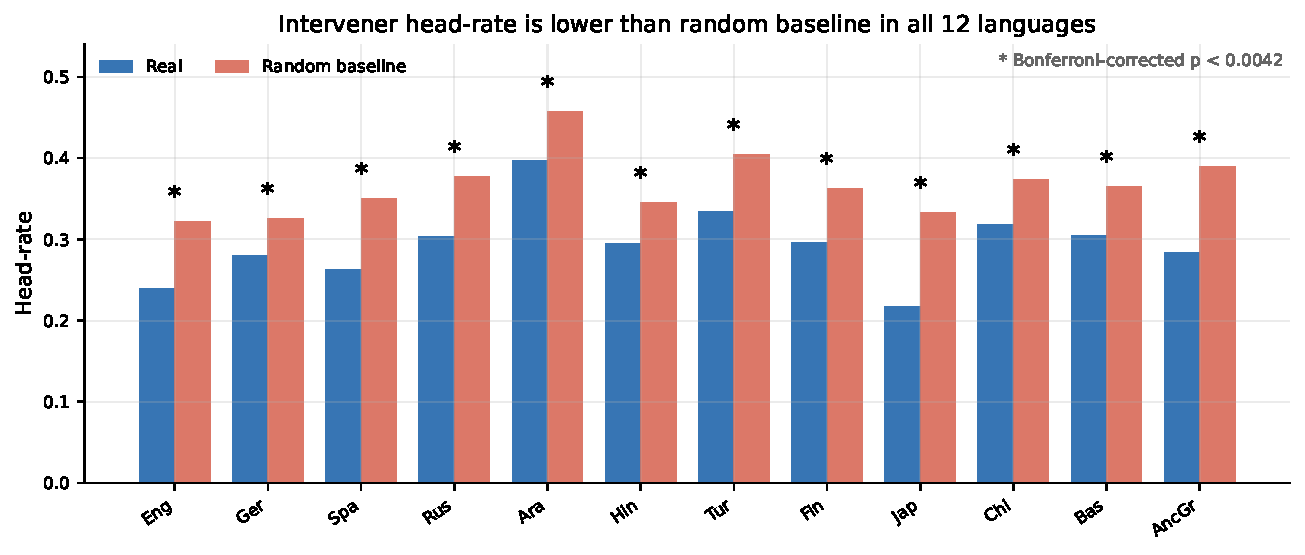
\includegraphics[width=0.92\linewidth]{data/figures/fig1_head_rate_comparison.pdf}
  \caption{Primary ICM result. In all 12 languages, the proportion of interveners that are syntactic heads is lower in real word order than in the random-linearisation baseline. Stars indicate Bonferroni-corrected significance.}
  \label{fig:headrate}
\end{figure}

\begin{figure}[H]
  \centering
  \begin{subfigure}{0.49\linewidth}
    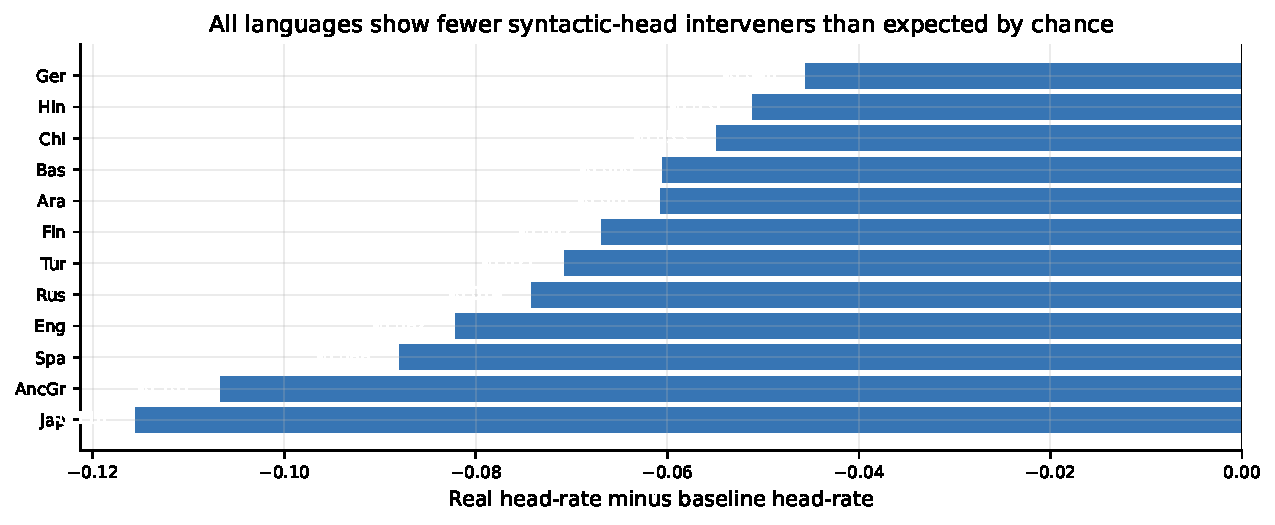
\includegraphics[width=\linewidth]{data/figures/fig2_head_rate_difference.pdf}
    \caption{Real minus baseline head-rate.}
  \end{subfigure}
  \begin{subfigure}{0.49\linewidth}
    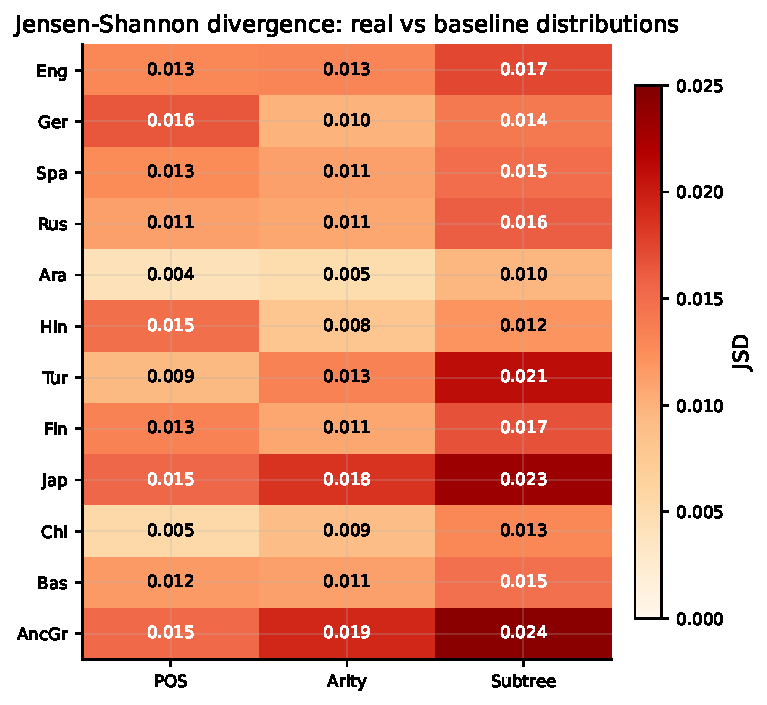
\includegraphics[width=\linewidth]{data/figures/fig3_jsd_heatmap.pdf}
    \caption{JSD by feature and language.}
  \end{subfigure}
  \caption{All languages show a negative head-rate difference. Distributional divergence is small in absolute size, but consistent across POS, arity, and subtree size.}
  \label{fig:diff-jsd}
\end{figure}

\begin{table}[H]
\centering
\small
\caption{Key statistical results. Head-rate tests compare real and baseline proportions. Arity and subtree p-values are from one-tailed Mann--Whitney U tests. All entries are significant at $\alpha=0.0042$.}
\resizebox{\linewidth}{!}{
\begin{tabular}{lrrrrr}
\toprule
Language & Real head & Base head & Difference & Arity $p$ & Subtree $p$ \\
\midrule
English & 0.240 & 0.322 & -0.082 & 1.35e-231 & 1.36e-236 \\
German & 0.280 & 0.326 & -0.046 & 9.44e-93 & 7.66e-97 \\
Spanish & 0.263 & 0.351 & -0.088 & 1.47e-235 & 4.50e-298 \\
Russian & 0.304 & 0.378 & -0.074 & 3.80e-179 & 3.06e-220 \\
Arabic & 0.397 & 0.458 & -0.061 & 7.69e-114 & 9.62e-152 \\
Hindi & 0.295 & 0.346 & -0.051 & 1.10e-100 & 6.14e-99 \\
Turkish & 0.334 & 0.405 & -0.071 & 3.17e-187 & 1.21e-235 \\
Finnish & 0.296 & 0.363 & -0.067 & 2.17e-169 & 1.52e-174 \\
Japanese & 0.218 & 0.333 & -0.116 & 0.00e+00 & 0.00e+00 \\
Chinese & 0.318 & 0.373 & -0.055 & 3.23e-103 & 3.07e-113 \\
Basque & 0.304 & 0.365 & -0.061 & 2.41e-151 & 1.94e-166 \\
Ancient Greek & 0.283 & 0.390 & -0.107 & 0.00e+00 & 0.00e+00 \\
\bottomrule
\end{tabular}}
\label{tab:main-results}
\end{table}

\begin{figure}[H]
  \centering
  \begin{subfigure}{0.49\linewidth}
    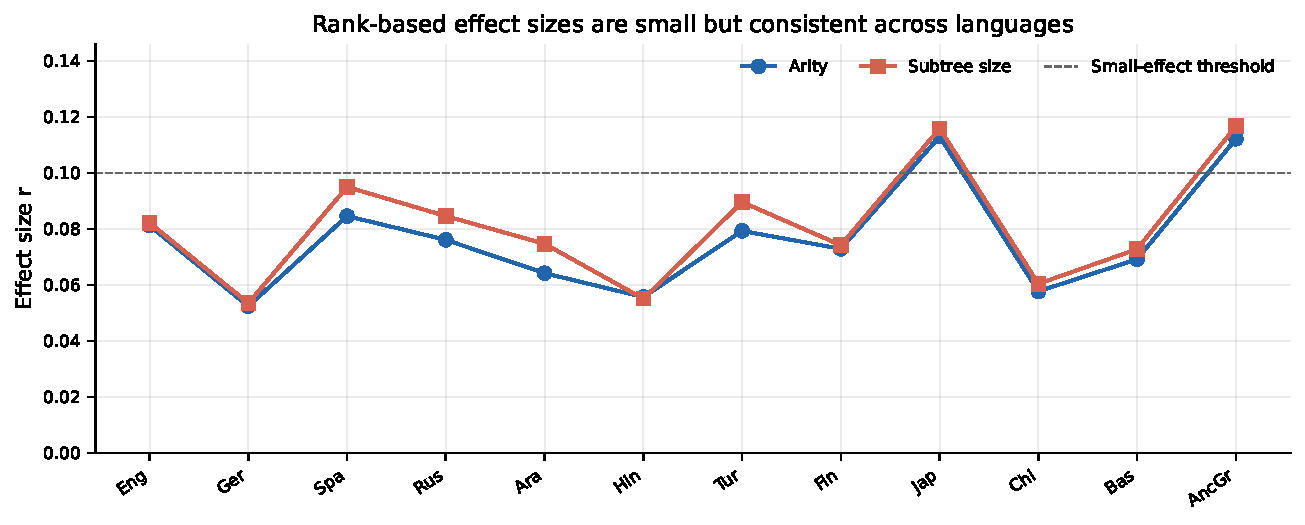
\includegraphics[width=\linewidth]{data/figures/fig4_mwu_effect_sizes.pdf}
    \caption{Rank-based effect sizes.}
  \end{subfigure}
  \begin{subfigure}{0.49\linewidth}
    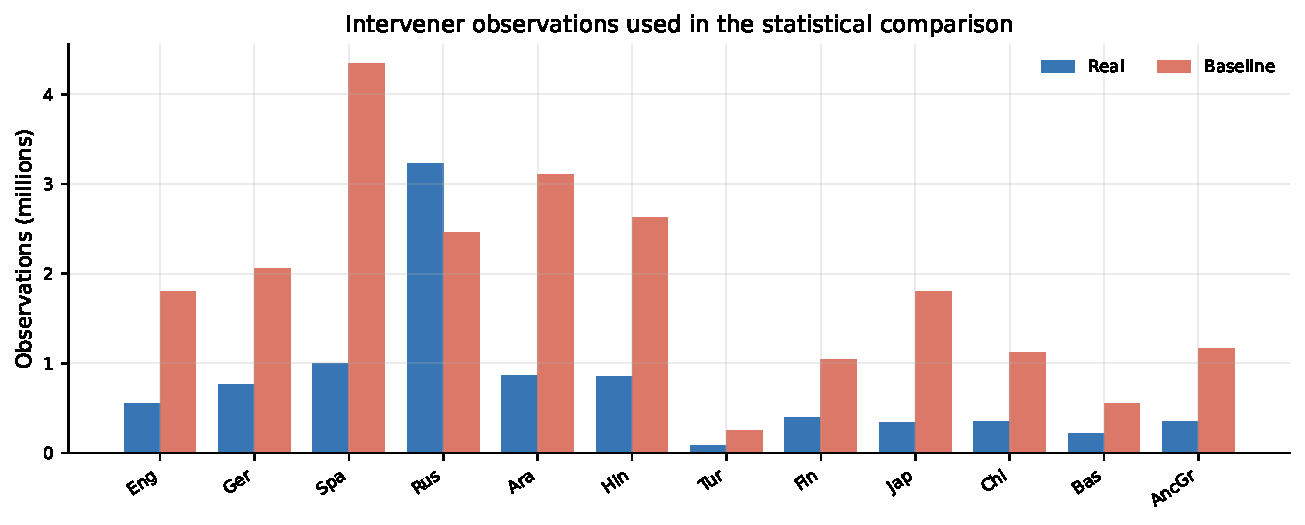
\includegraphics[width=\linewidth]{data/figures/fig5_sample_sizes.pdf}
    \caption{Observation counts.}
  \end{subfigure}
  \caption{The statistical effects are small to modest in size, but they are extremely consistent and are estimated from large samples. Arity effect sizes range from 0.052 to 0.113; subtree effect sizes range from 0.054 to 0.117.}
  \label{fig:effects-samples}
\end{figure}

The JSD values are low in absolute magnitude: POS ranges from 0.0043 to 0.0165, arity from 0.0050 to 0.0193, and subtree size from 0.0097 to 0.0243. This means real and baseline distributions are not radically different overall. The important result is directional consistency: every language has lower real head-rate, lower arity, and lower subtree size than expected under the random baseline.

\section{Theoretical Implications}
The results support the idea that dependency locality is not only about linear distance. Languages also appear to manage the syntactic complexity of the material placed between related words. This is compatible with memory-based theories of processing: intervening syntactic heads can introduce additional incomplete dependencies and increase retrieval interference, so avoiding them should make sentence comprehension easier.

The findings also suggest a possible bridge between DLM and richer theories of word order. DLM predicts shorter dependencies; ICM predicts simpler material inside dependencies. These pressures can work together, but they are not identical. A language might allow a long dependency when the intervening material is simple, while avoiding long spans that contain complex phrase structure. This helps explain why distance-based metrics alone may miss part of the processing pressure shaping word order.

The effects are not large, so they should not be interpreted as a deterministic grammar rule. They are better understood as a statistical pressure visible across large corpora. The consistency across 12 languages, including typologically different languages, suggests that ICM is a plausible cross-linguistic tendency relevant to both human language processing and machine models of syntax.

\clearpage
\bibliographystyle{plain}
\begin{thebibliography}{9}
\bibitem{gibson1998linguistic}
Gibson, E. (1998).
\newblock Linguistic complexity: Locality of syntactic dependencies.
\newblock \emph{Cognition}, 68(1), 1--76.

\bibitem{liu2008dependency}
Liu, H. (2008).
\newblock Dependency distance as a metric of language comprehension difficulty.
\newblock \emph{Journal of Cognitive Science}, 9(2), 159--191.

\bibitem{nivre2020universal}
Nivre, J., de Marneffe, M.-C., Ginter, F., Haji\v{c}, J., Manning, C. D.,
Pyysalo, S., Schuster, S., Tyers, F., and Zeman, D. (2020).
\newblock Universal Dependencies v2: An evergrowing multilingual treebank collection.
\newblock \emph{Proceedings of LREC}.

\bibitem{yadav2022reappraisal}
Yadav, H., Mittal, S., and Husain, S. (2022).
\newblock A reappraisal of dependency length minimization as a linguistic universal.
\newblock \emph{Open Mind}, 6, 147--168.
\newblock \url{https://doi.org/10.1162/opmi_a_00060}.
\end{thebibliography}

\clearpage
\appendix
\section{Implementation Details}
\textbf{Pipeline.} The implementation is organised as a reproducible sequence of scripts:
\begin{enumerate}
  \item \texttt{step2\_verify\_data.py}: validate CoNLL-U files.
  \item \texttt{step3\_extract\_interveners.py}: extract one row per arc-intervener pair.
  \item \texttt{step4\_compute\_features.py}: aggregate POS, arity, subtree, attachment, and head-rate statistics.
  \item \texttt{step5\_baseline\_generator.py}: build the random-linearisation baseline.
  \item \texttt{step6\_statistical\_tests.py}: run JSD, Mann--Whitney U, and head-rate tests.
  \item \texttt{step7\_visualizations.py}: generate the full figure set.
\end{enumerate}

\textbf{Core extraction code.} The following excerpt implements the formal definition of an intervener and records the four project features.
\lstinputlisting[firstline=114,lastline=227]{step3_extract_interveners.py}

\textbf{Inference code.} The statistical script implements the following logic; the full runnable version is in \texttt{step6\_statistical\_tests.py}.
\begin{lstlisting}[language=Python]
def jensen_shannon_divergence(p, q):
    m = [0.5 * (pi + qi) for pi, qi in zip(p, q)]
    jsd = 0.5 * kl_divergence(p, m) + 0.5 * kl_divergence(q, m)
    return jsd / math.log(2)  # convert to bits

def mann_whitney_test(real_sample, baseline_sample):
    # One-tailed test: real values are lower than baseline values.
    u_stat, p_value = stats.mannwhitneyu(
        real_sample, baseline_sample, alternative="less"
    )
    n1, n2 = len(real_sample), len(baseline_sample)
    mean_u = n1 * n2 / 2
    std_u = math.sqrt(n1 * n2 * (n1 + n2 + 1) / 12)
    z_score = (u_stat - mean_u) / std_u
    effect_r = abs(z_score) / math.sqrt(n1 + n2)
    return p_value, effect_r
\end{lstlisting}

\clearpage
\section{Complete Figure Appendix}
The main report uses the most compact result figures. The remaining generated figures from \texttt{data/figures} are included here for completeness.

\begin{figure}[H]
  \centering
  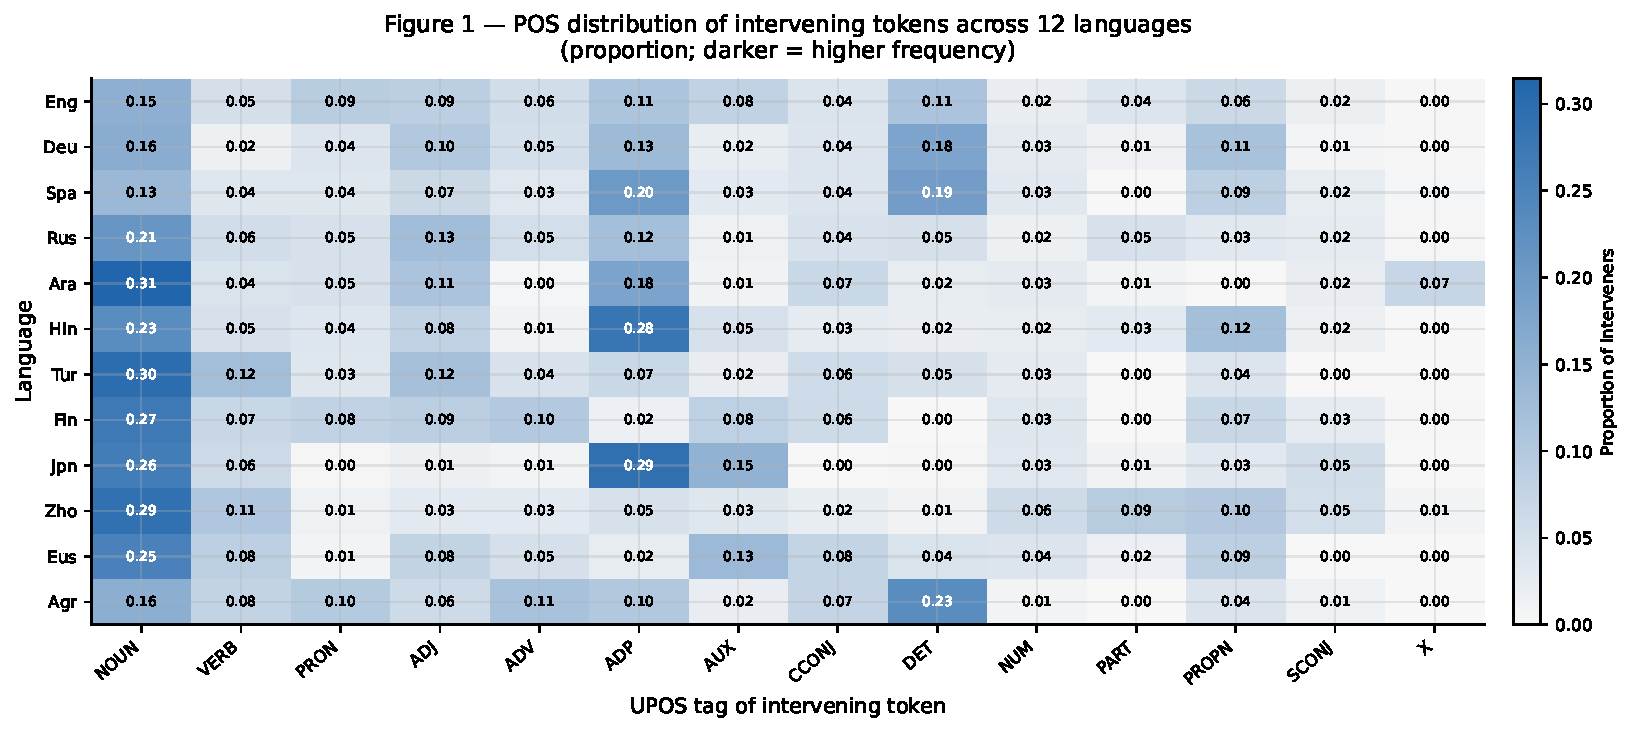
\includegraphics[width=0.95\linewidth]{data/figures/fig1_pos_heatmap.pdf}
  \caption{Original project Figure 1: POS distribution heatmap.}
\end{figure}

\begin{figure}[H]
  \centering
  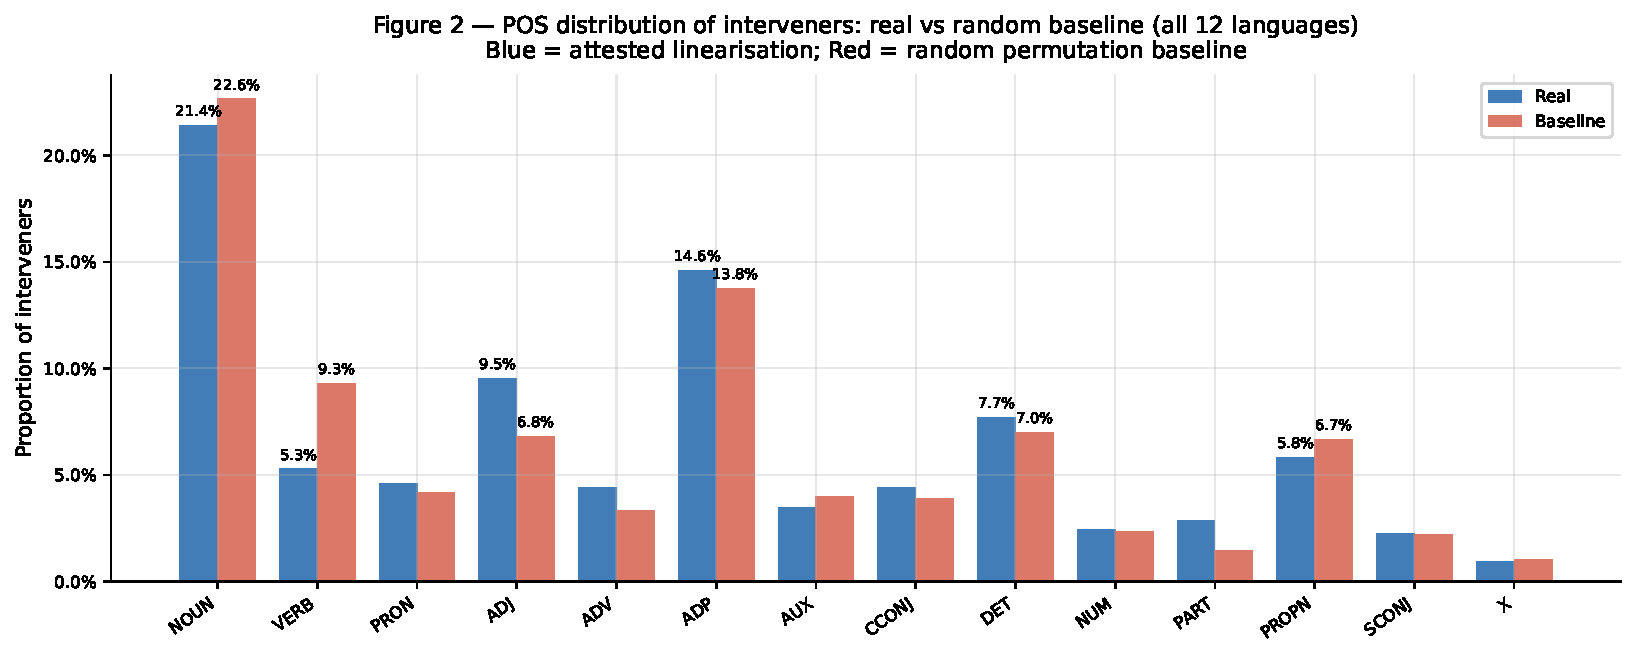
\includegraphics[width=0.95\linewidth]{data/figures/fig2_pos_bar_real_vs_baseline.pdf}
  \caption{Original project Figure 2: POS distribution, real versus baseline.}
\end{figure}

\begin{figure}[H]
  \centering
  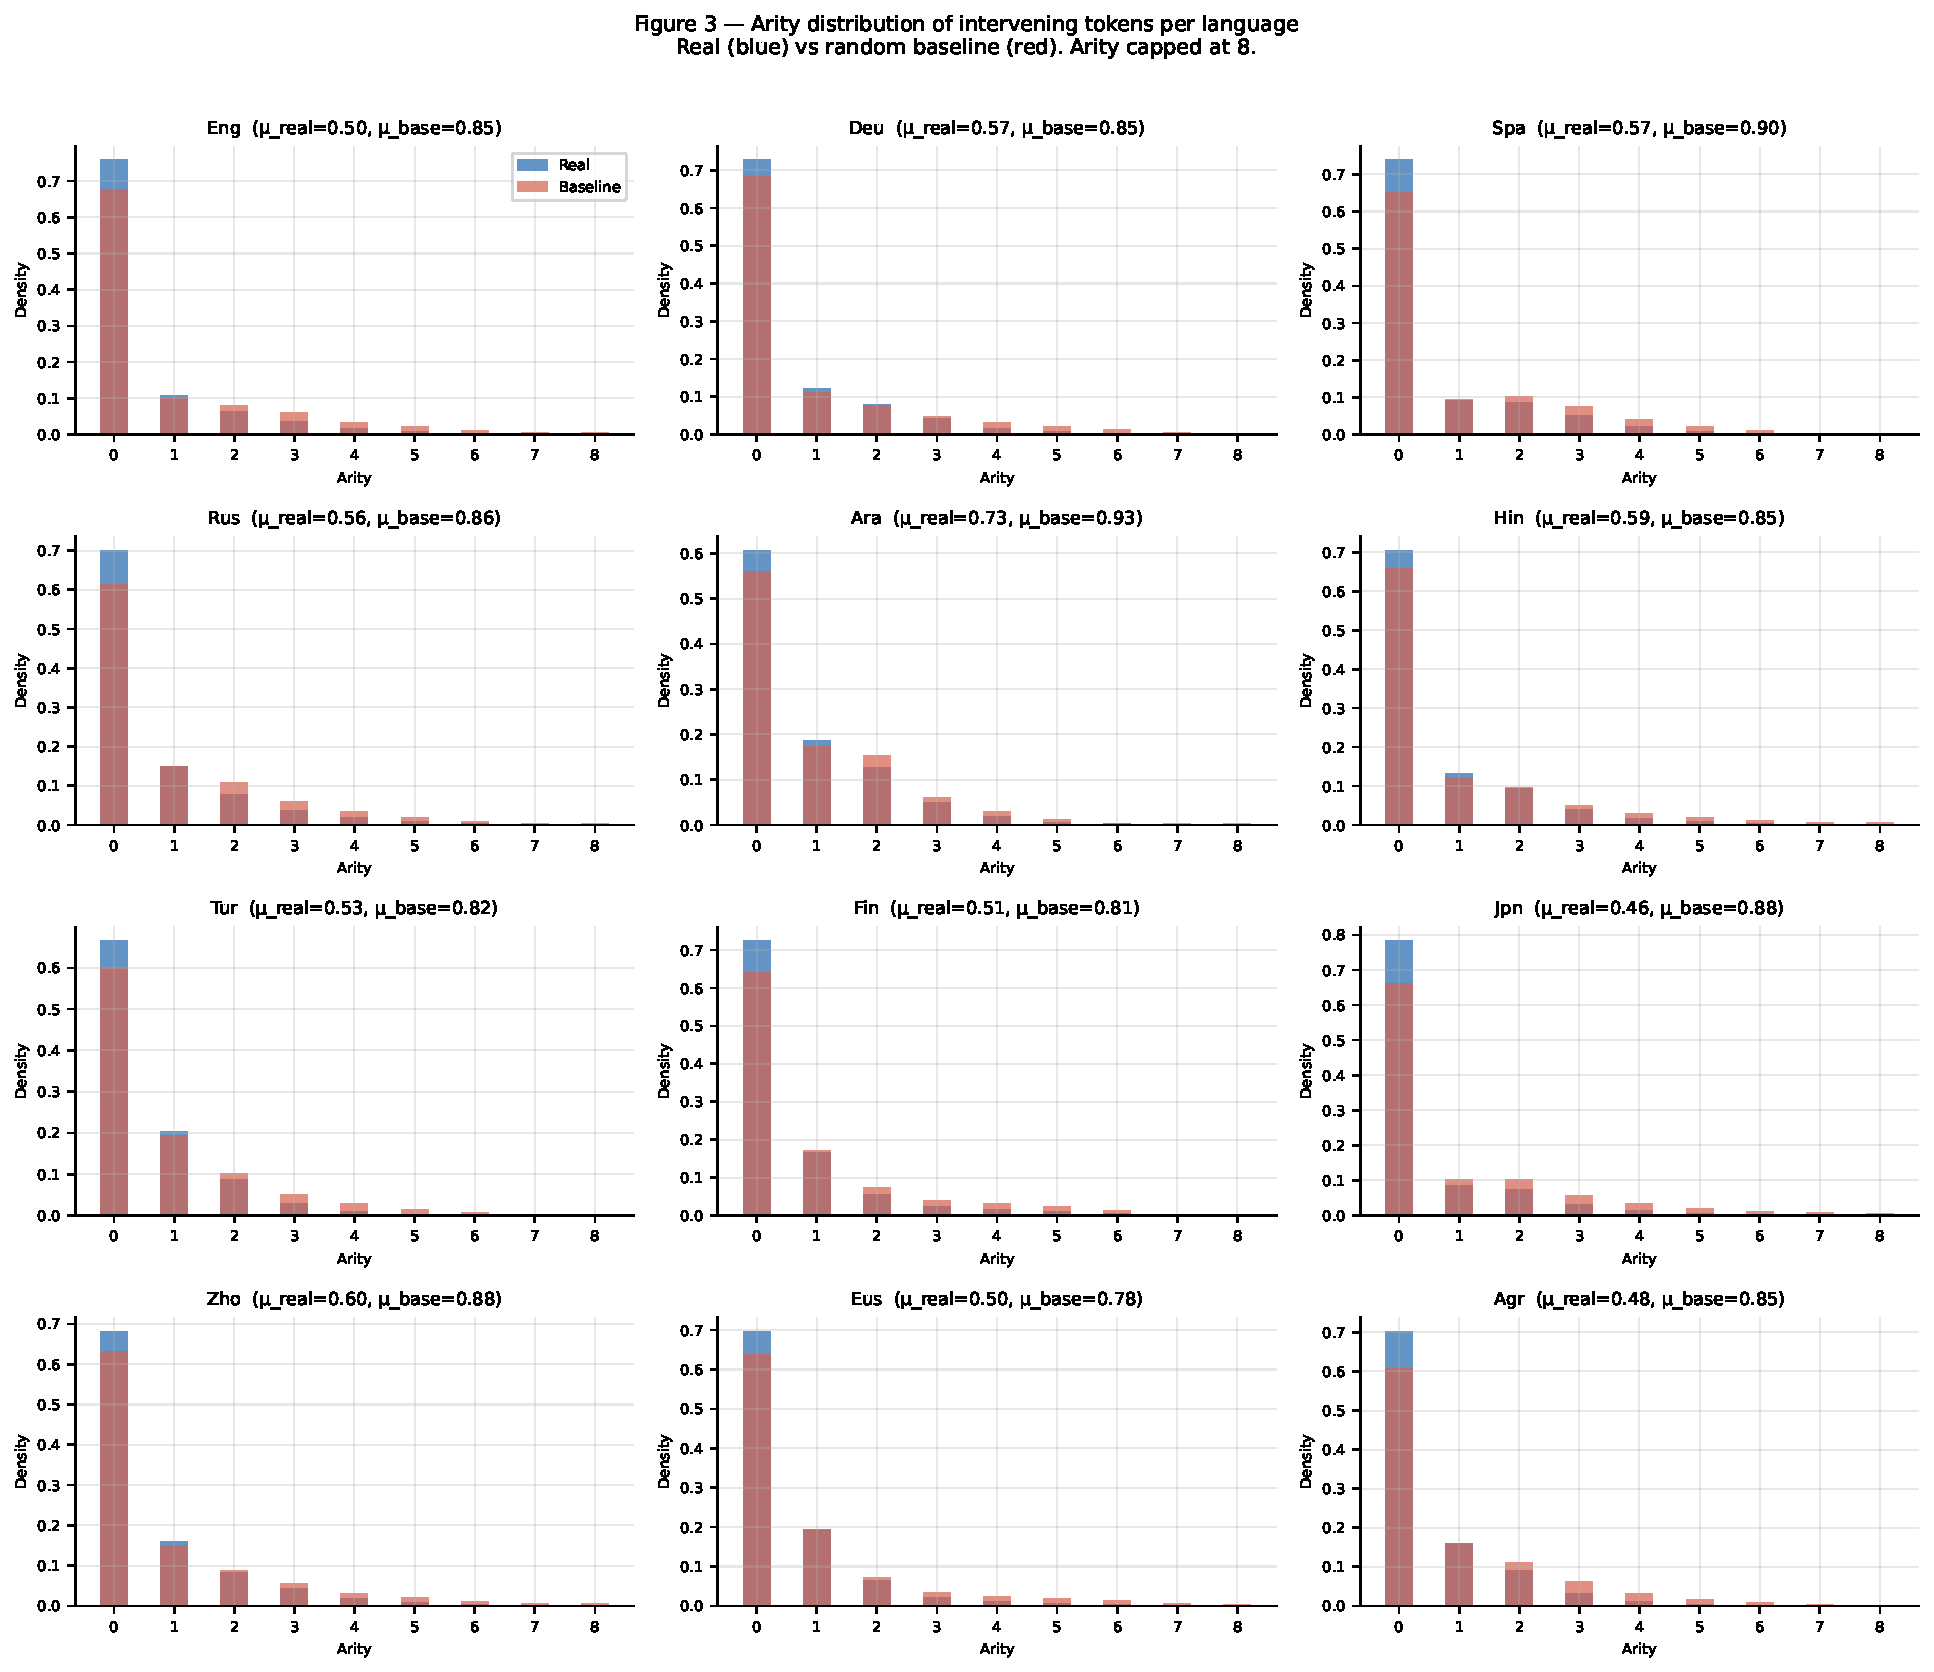
\includegraphics[width=0.95\linewidth]{data/figures/fig3_arity_grid.pdf}
  \caption{Original project Figure 3: arity distributions by language.}
\end{figure}

\begin{figure}[H]
  \centering
  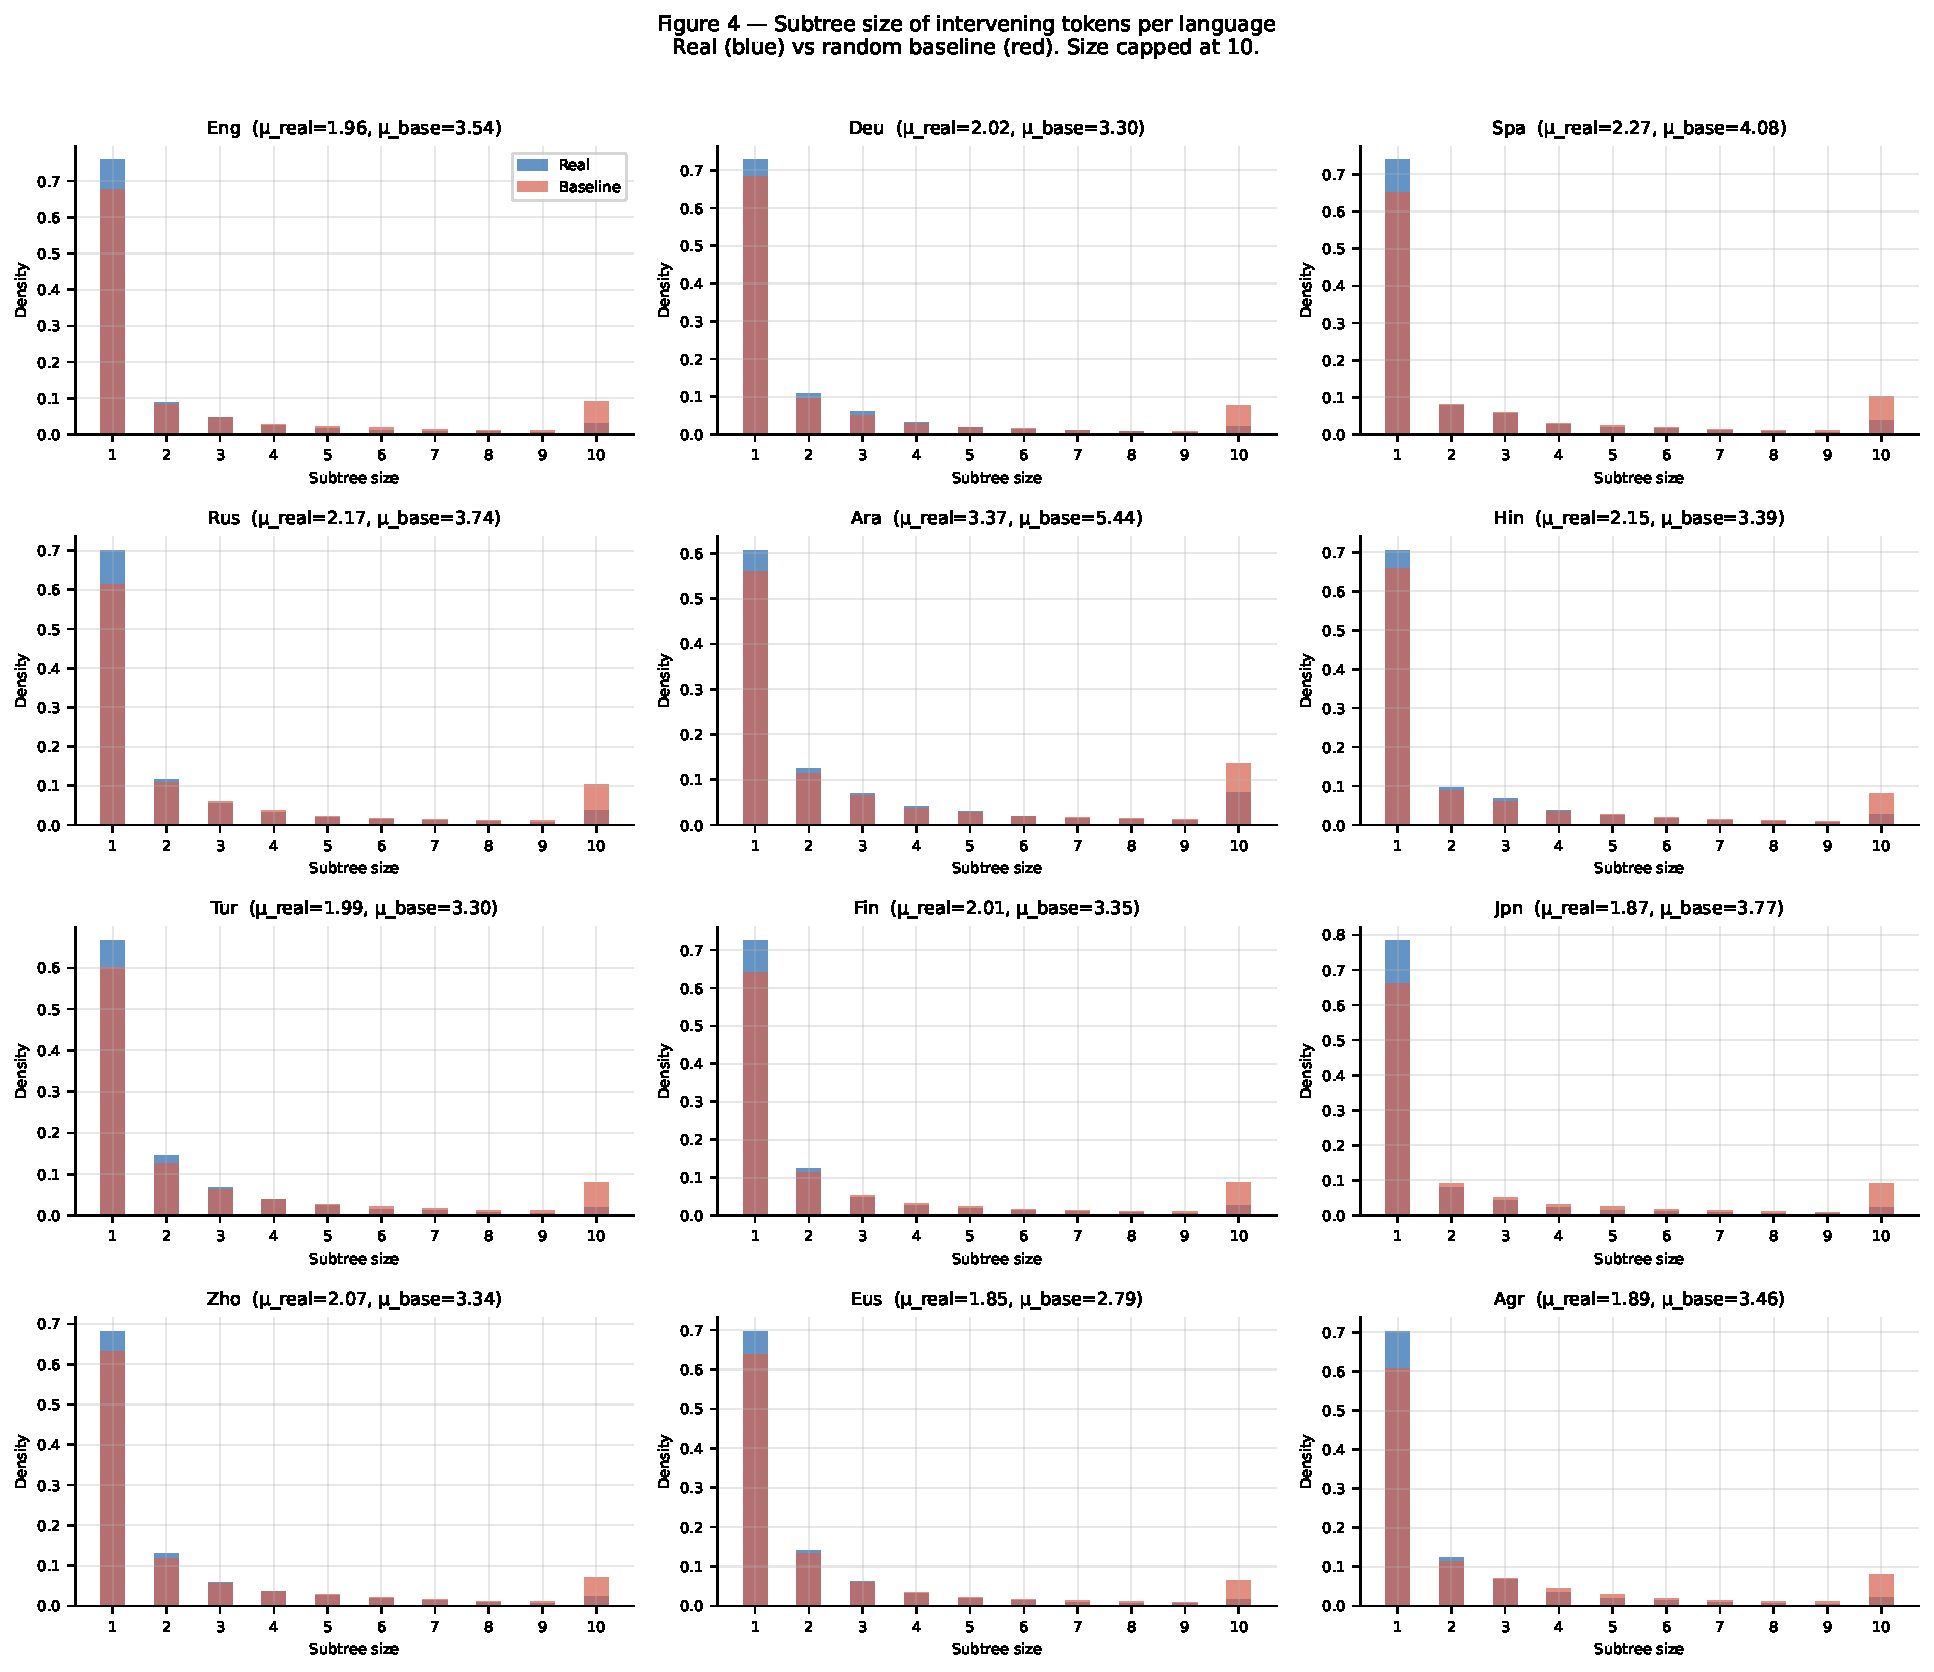
\includegraphics[width=0.95\linewidth]{data/figures/fig4_subtree_grid.pdf}
  \caption{Original project Figure 4: subtree-size distributions by language.}
\end{figure}

\begin{figure}[H]
  \centering
  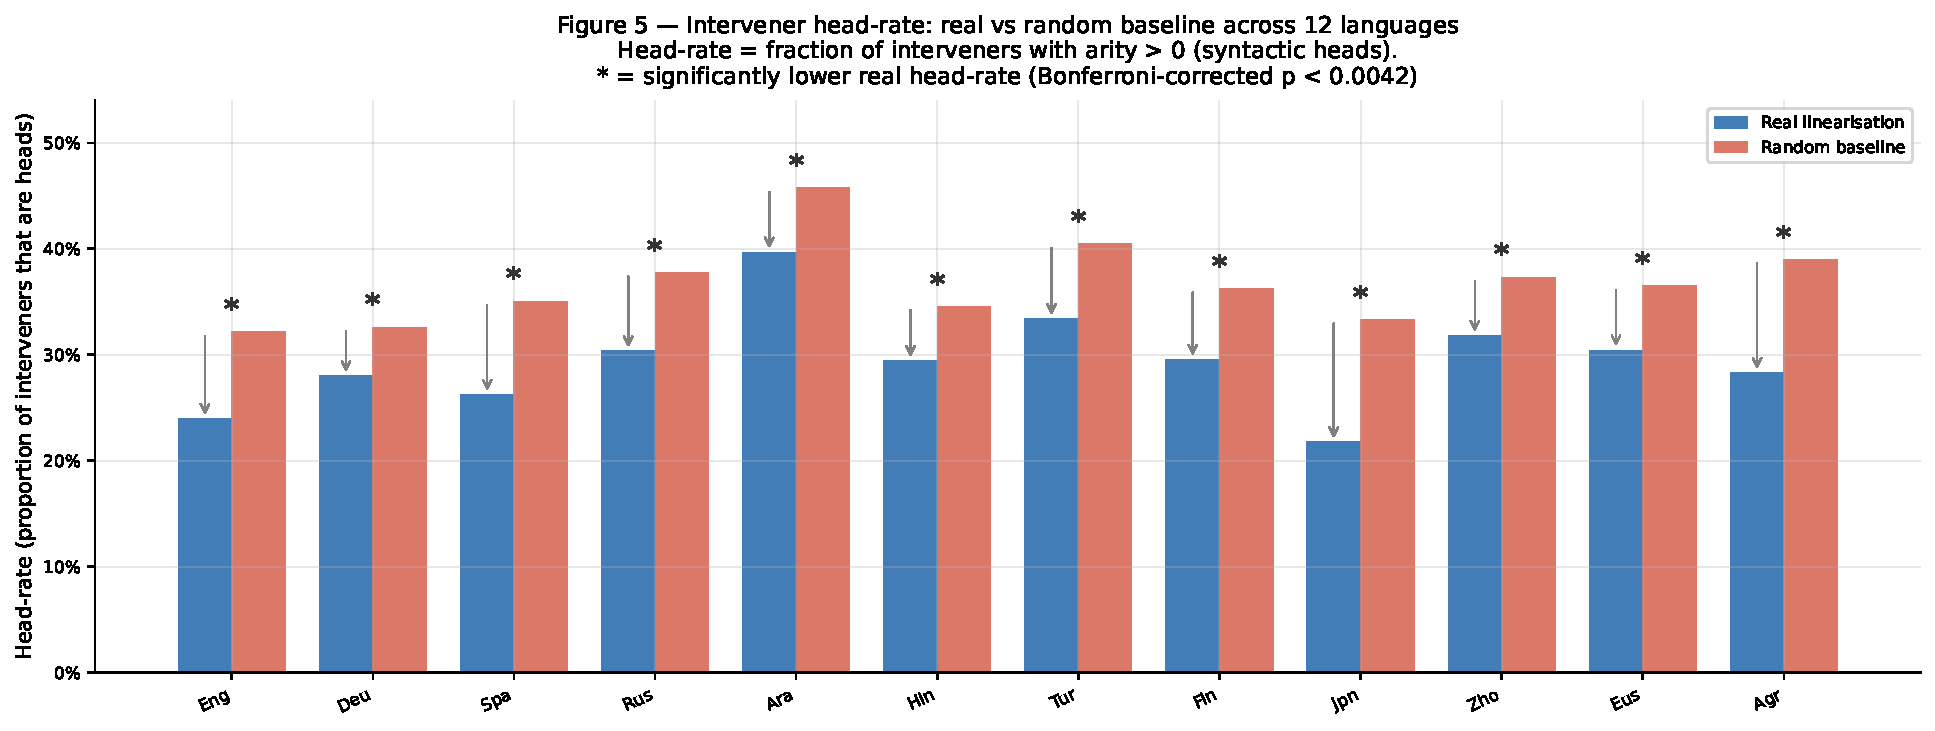
\includegraphics[width=0.95\linewidth]{data/figures/fig5_head_rate_comparison.pdf}
  \caption{Original project Figure 5: head-rate comparison.}
\end{figure}

\begin{figure}[H]
  \centering
  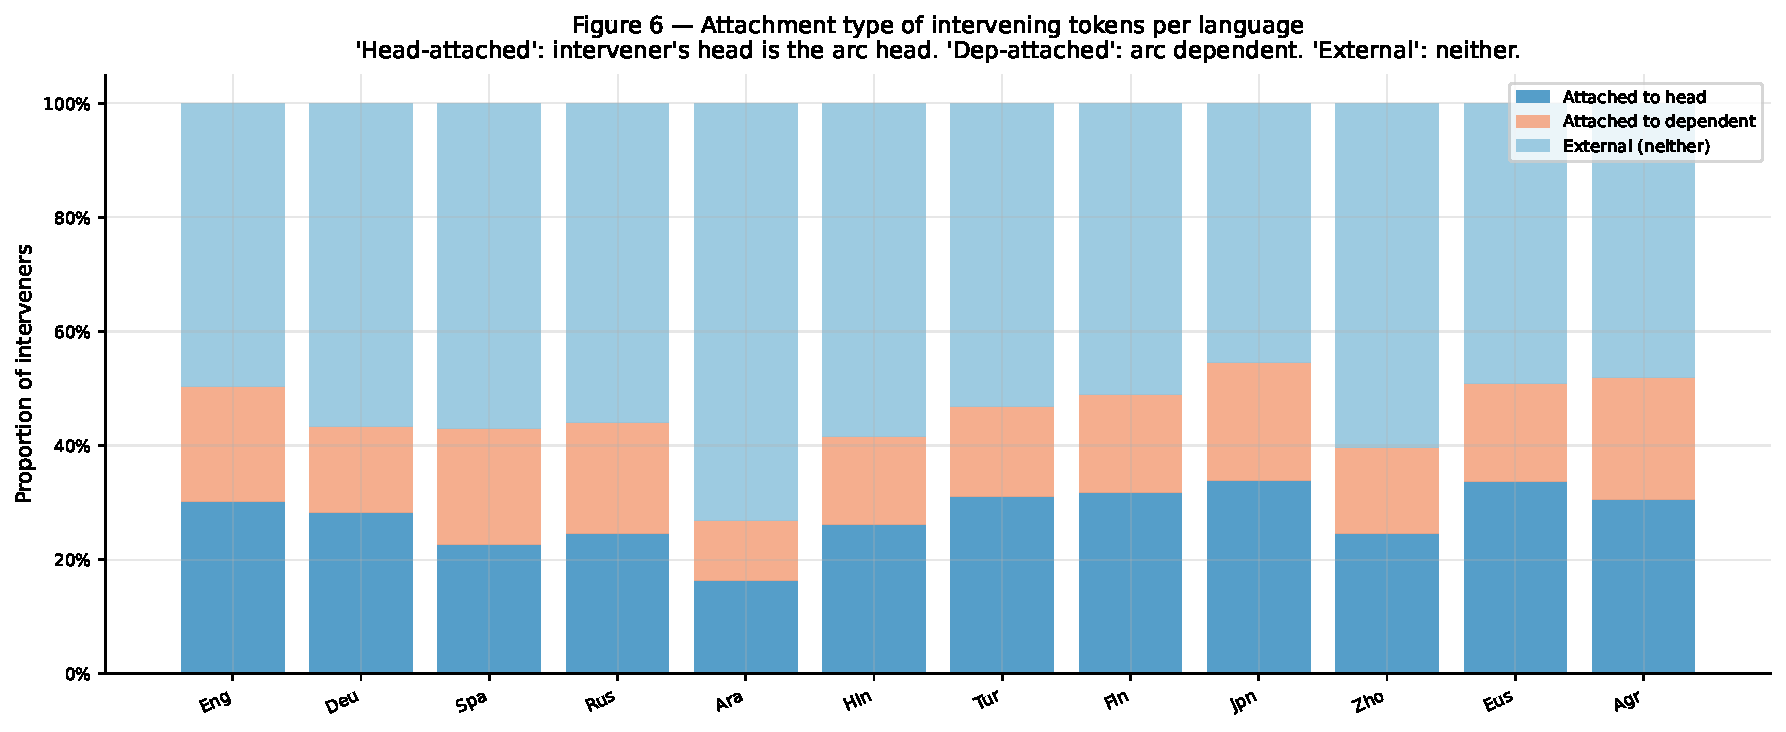
\includegraphics[width=0.95\linewidth]{data/figures/fig6_attachment_stacked.pdf}
  \caption{Original project Figure 6: attachment type distribution.}
\end{figure}

\begin{figure}[H]
  \centering
  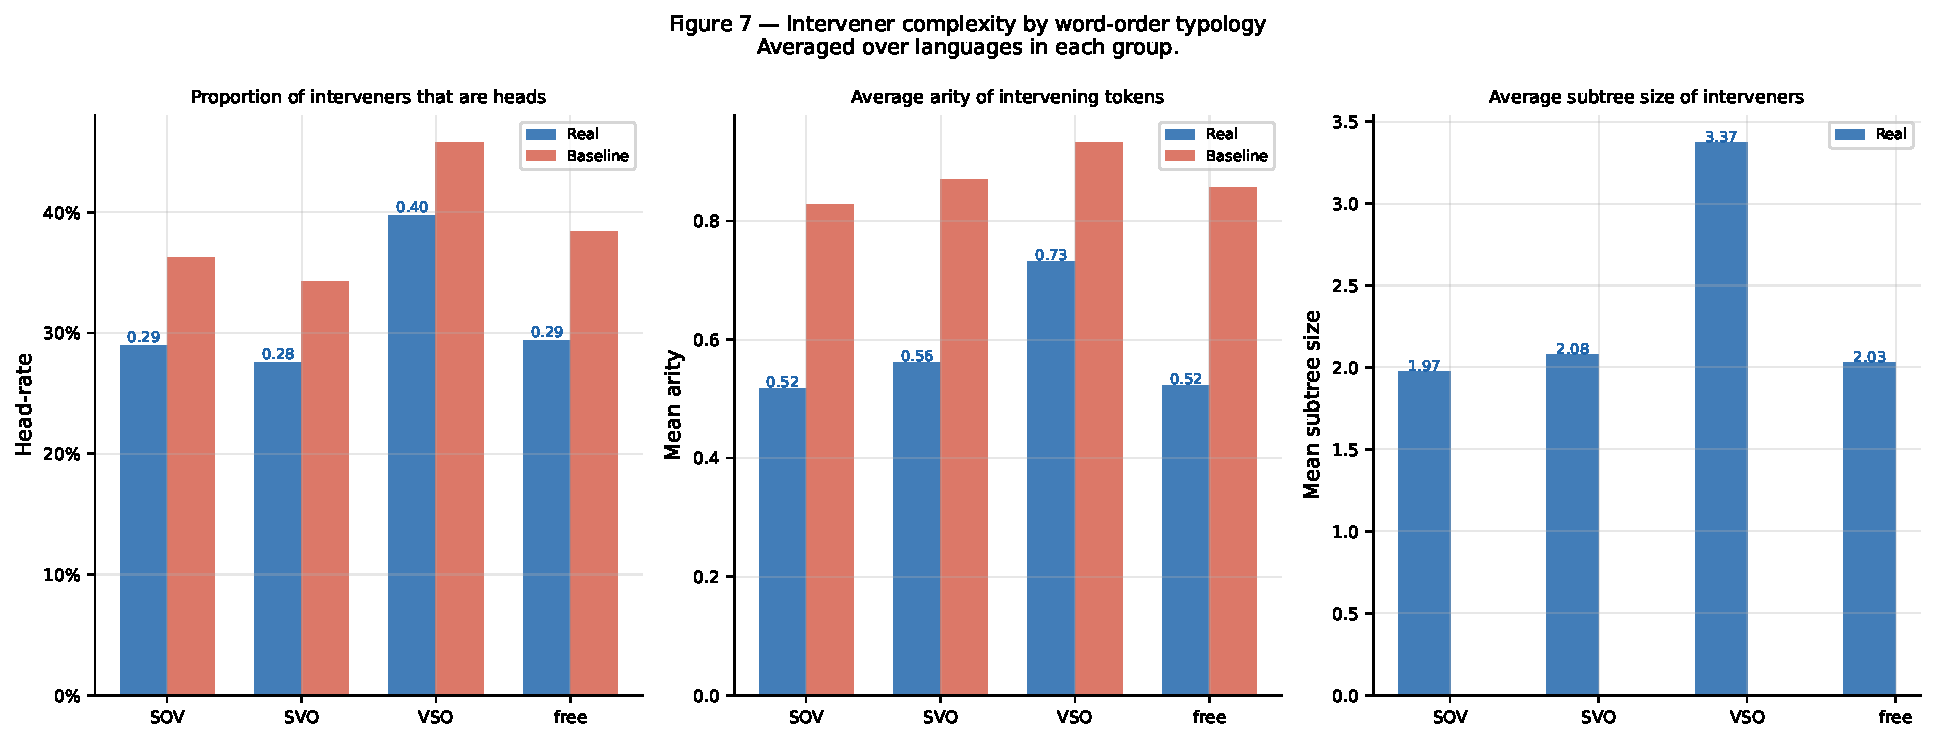
\includegraphics[width=0.95\linewidth]{data/figures/fig7_word_order_comparison.pdf}
  \caption{Original project Figure 7: word-order group comparison.}
\end{figure}

\begin{figure}[H]
  \centering
  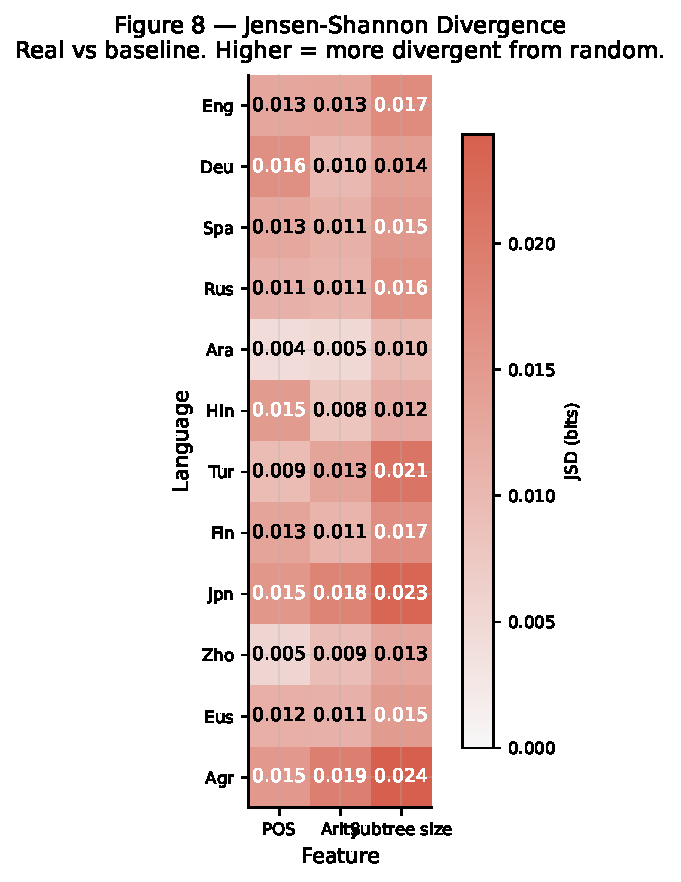
\includegraphics[width=0.82\linewidth]{data/figures/fig8_jsd_heatmap.pdf}
  \caption{Original project Figure 8: JSD heatmap.}
\end{figure}

\begin{figure}[H]
  \centering
  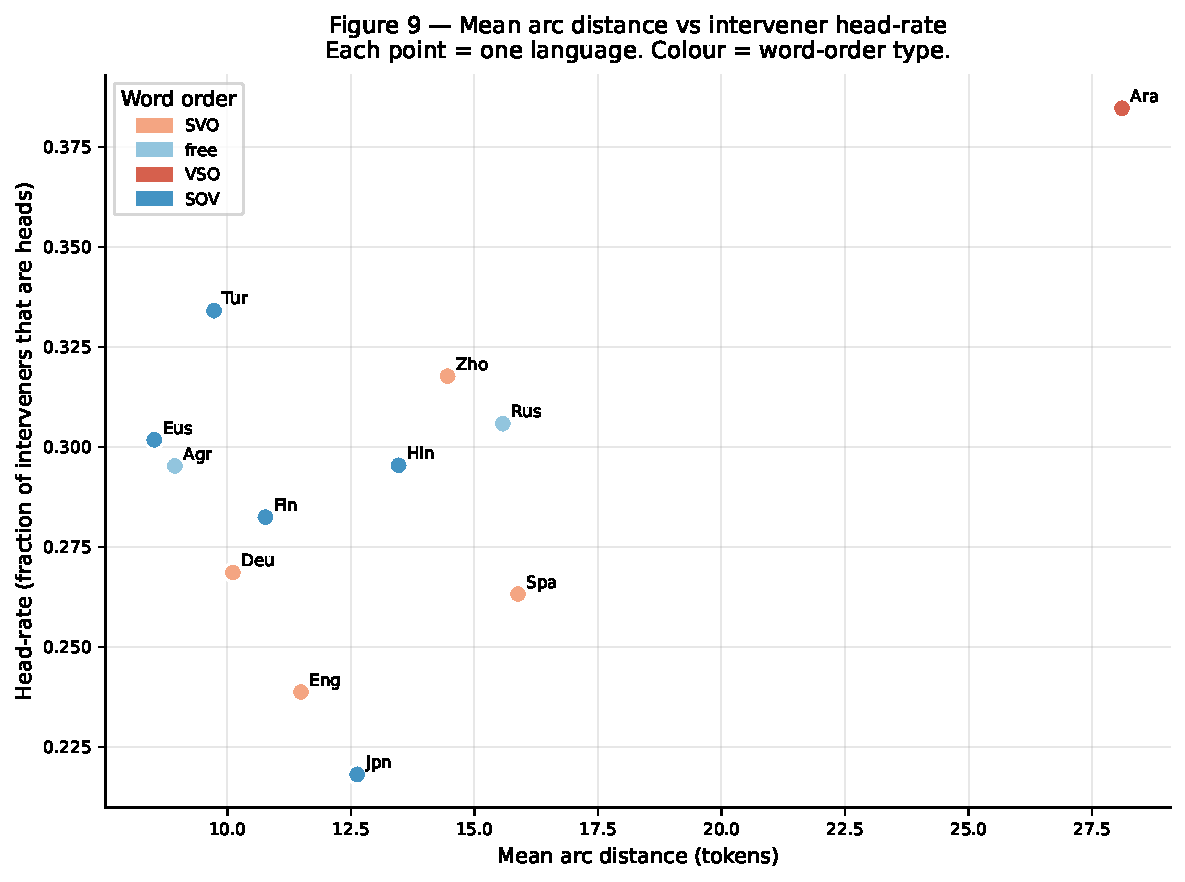
\includegraphics[width=0.82\linewidth]{data/figures/fig9_arc_vs_headrate_scatter.pdf}
  \caption{Original project Figure 9: mean arc distance versus intervener head-rate.}
\end{figure}

\begin{figure}[H]
  \centering
  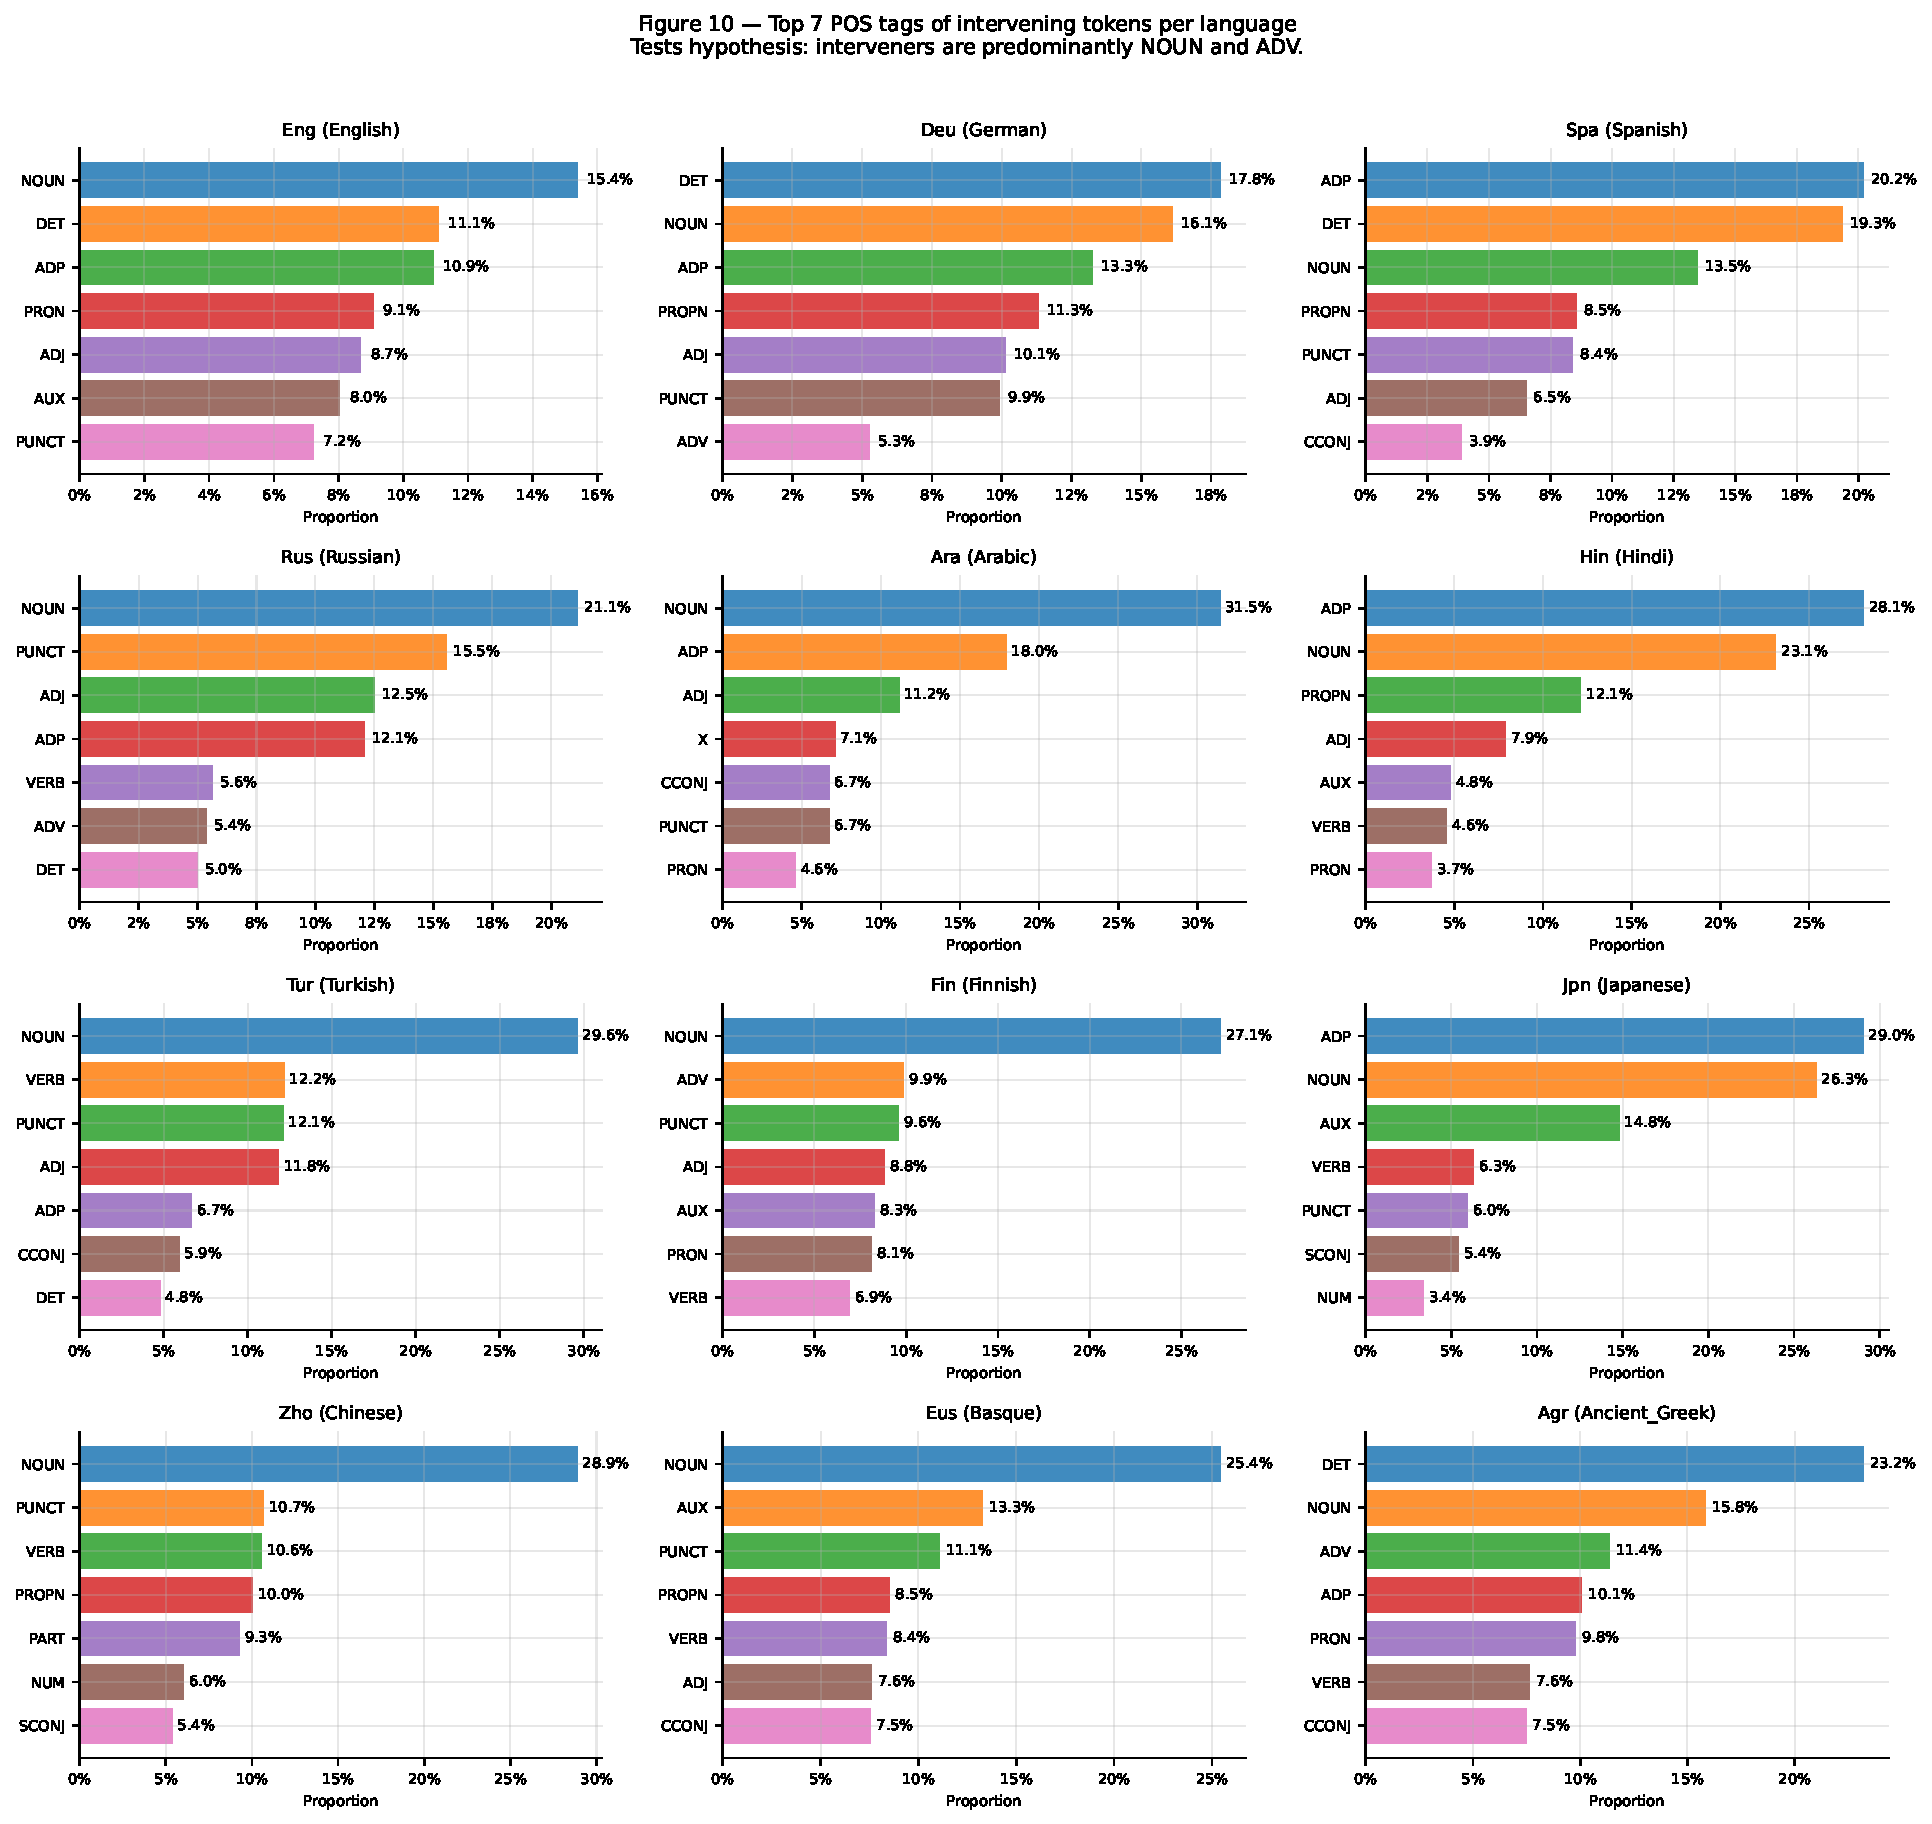
\includegraphics[width=0.95\linewidth]{data/figures/fig10_top_pos_per_language.pdf}
  \caption{Original project Figure 10: top POS tags of interveners by language.}
\end{figure}

\end{document}
